\section{Технологическая часть}

В данном разделе будет обоснован выбор средств программной реализации предлагаемого метода, описан формат входных и выходных данных. 
Разработано программное обеспечение, реализующее представленный метод, приведен пример работы программы, выполнено тестирование, а также описан способ обращения к программе.

\subsection{Выбор средств разработки}

\subsubsection{Выбор платформы}
По результатам анализа только исследуемые методы отображения интерфейса нативной мобильной разработки не обладают функцией горячей перезагрузки. 
В связи с чем в качестве платформы разработки для реализации предлагаемого метода выбрана операционная система iOS.

\subsubsection{Выбор языка программирования}
Выбран язык Swift \cite{swift}, поскольку он является основным используемым в нативной разработке iOS.

\subsubsection{Выбор среды разработки и сборка программного обеспечения}
Среда разработки --- XCode \cite{xcode}, поскольку является интегрированной средой разработки программного обеспечения для платформ macOS, iOS, watchOS и tvOS, разработанной корпорацией Apple, а также предоставляет возможность запуска разрабатываемого программного обеспечения на симуляторах устройств \cite{simulator}. 
Используется версия XCode 15.3, являющаяся актуальной на момент написания дипломной работы.
Запуск разрабатываемого программного обеспечения происходит на симуляторе устройства iPhone 15 Pro Max, версия iOS --- 17.4 (также является актуальной на момент написания дипломной работы).

\subsubsection{Используемые расширения}
Для создания представлений используется библиотека UIKit, содержащая полный набор базовых UI--элементов, а также механизмы размещения их на экране. 

\subsection{Формат входных и выходных данных}
Входные данные для разрабатываемого метода:

\begin{itemize}[label=---]
	\item пользовательский интерфейс;
	\item событие, инициализирующее изменения интерфейса;
	\item XML--файл, организованный специальным образом.
\end{itemize}

Выходные данные для разрабатываемого метода:

\begin{itemize}[label=---]
	\item пользовательский интерфейс, измененный во время выполнения программы.
\end{itemize}

\subsection{Способ обращения к программе}

Разработанная реализация метода представляет собой класс.
Для использования методов класса необходимо разместить файлы с кодом разработанного метода рядом с файлами программы. 
Для корректной работы приложения необходимо, чтобы каждый UIViewController, интерфейс которого будет реализован с помощью разработанного метода, был унаследован от класса, описанного в листинге 2. 

\begin{lstlisting}[caption={Класс, от которого наследуется UIViewController}]

class LayoutInTimeViewController: UIViewController {
    let fileManager = FileManager.default
    let layoutInTime = LayoutInTime()
    var filePath: String?

    func reload() {
        clearView(self.view)
        layoutInTime.createLayout(rootView: self.view, from: xmlString)
    }

    private func clearView(_ view: UIView) {
        for subview in view.subviews {
            subview.removeFromSuperview()
        }
    }
}
\end{lstlisting}

Для обновления интерфейса необходимо вызвать метод reload в методе жизненного цикла ViewDidLoad.

Также необходимо, чтобы UIViewController был внесен в список наблюдаемых объектов. Для этого необходимо добавить в метод жизненного цикла ViewDidLoad строку, представленную в листинге 3.

\begin{lstlisting}[caption={Внесение UIViewController в список наблюдаемых объектов}]
ReloadManager.addObserver(self)
\end{lstlisting}

Далее часть интерфейса или полностью весь интерфейс может быть спроектирован путем создания разметки XML--файла, связанного с UIViewController.

\subsubsection{Пример работы}

В качестве примера работы программного обеспечения был спроектирован интерфейс, содержащий фоновое представление белого цвета, на котором по центру располагается UILabel с текстом <<Привет!>>. 
Скриншот представлен на рисунке \ref{fig:example-before}.

\begin{figure}[!htb]
	\centering
	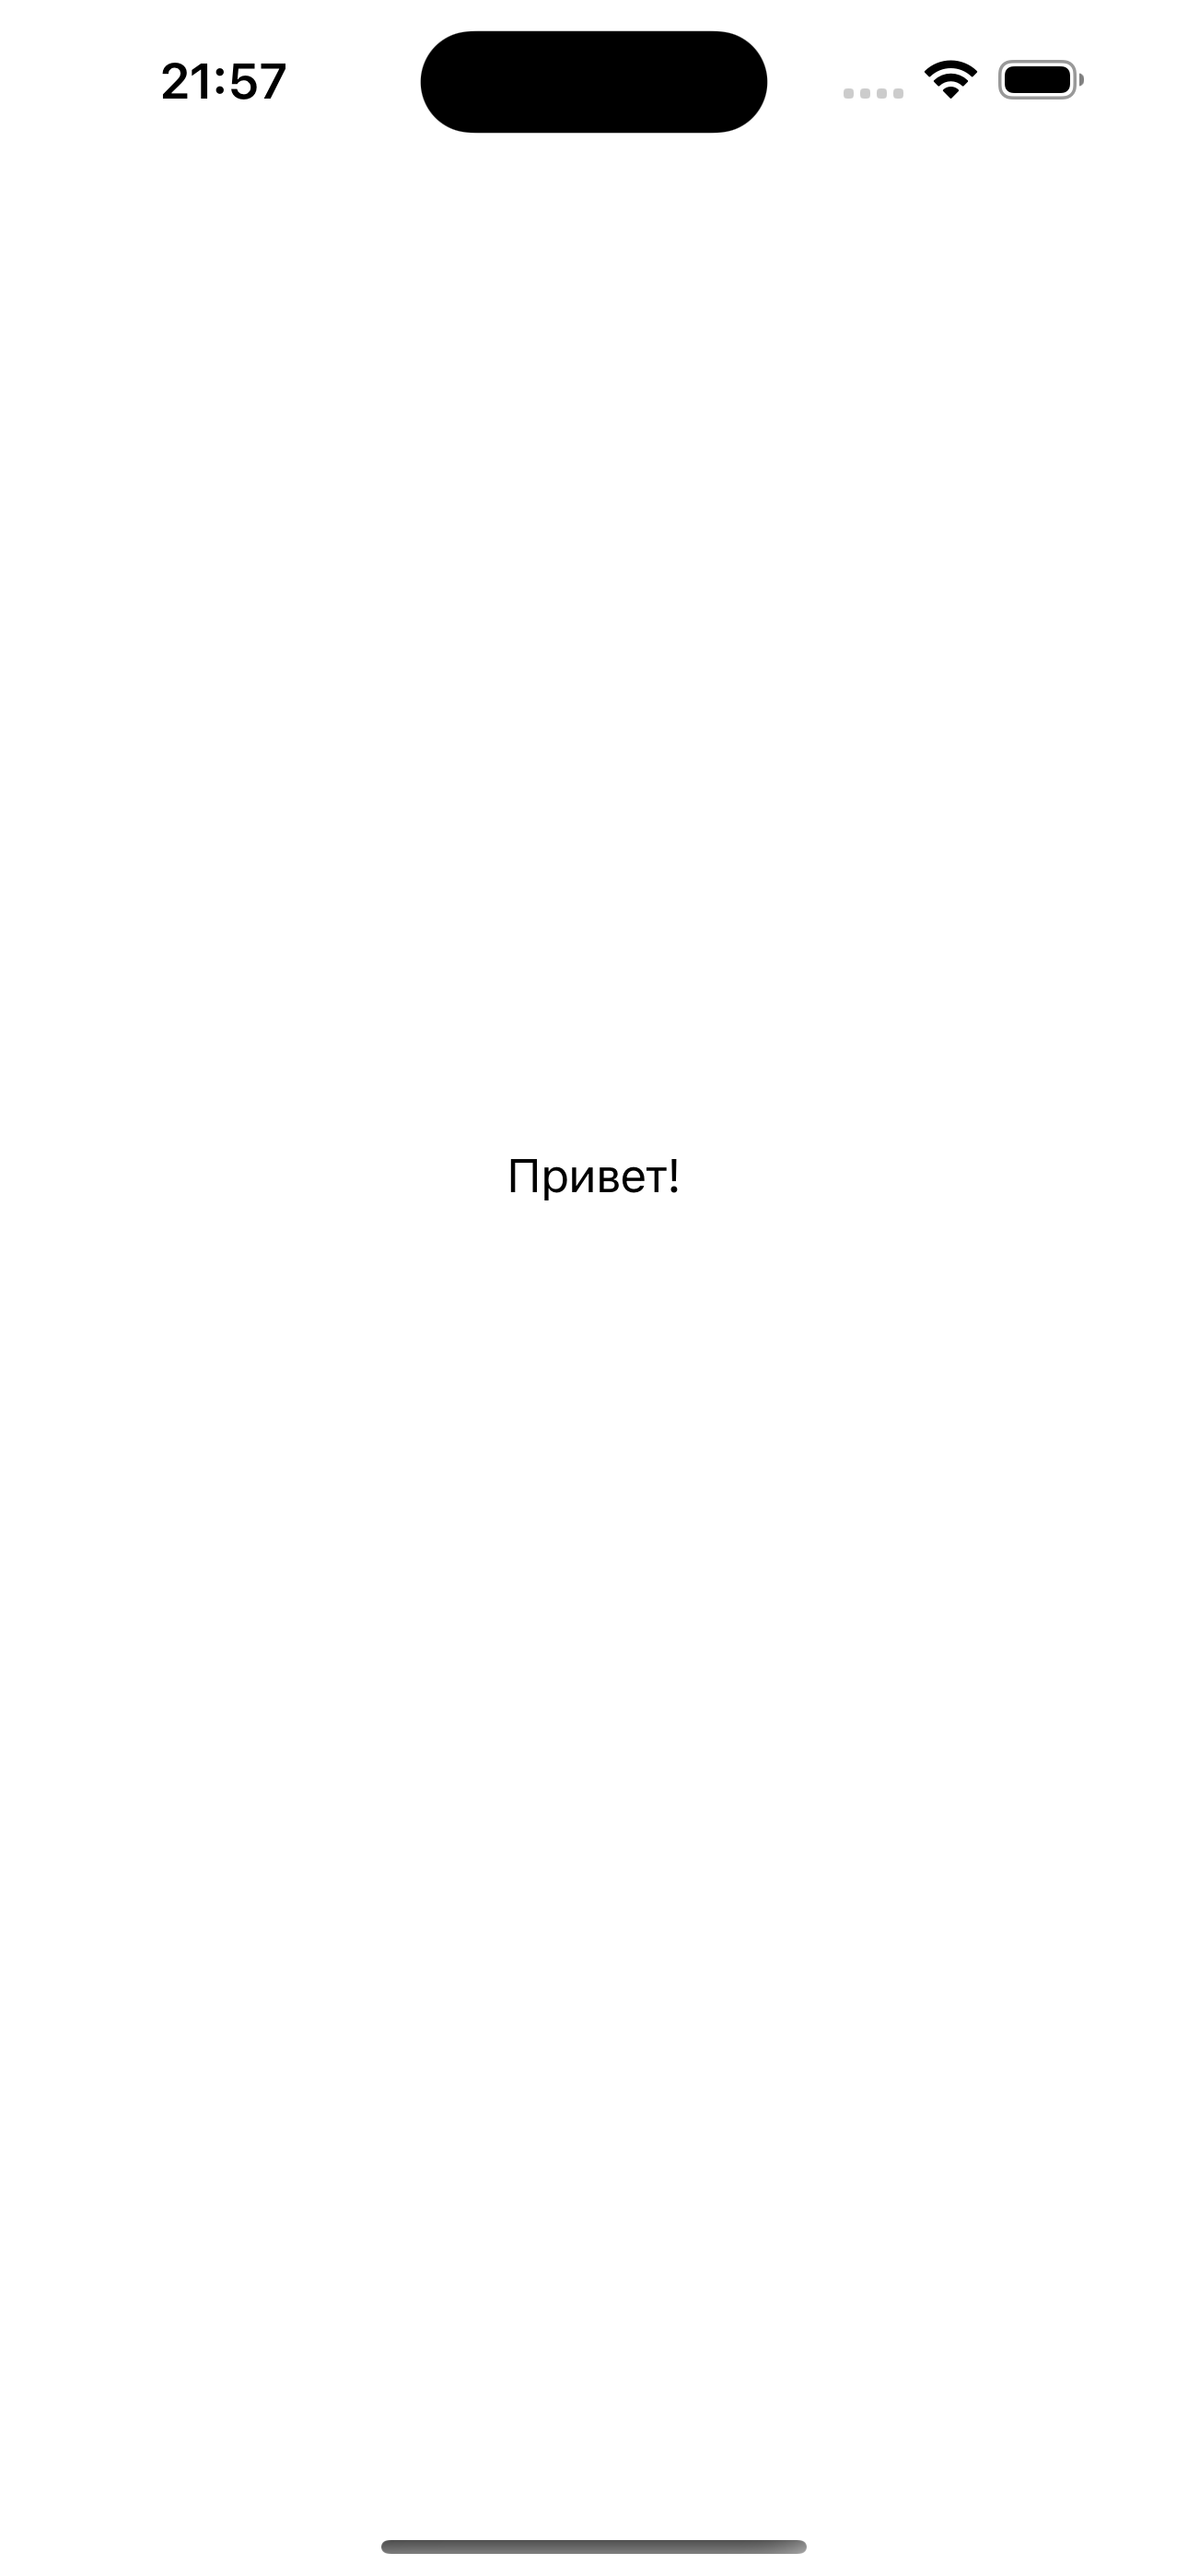
\includegraphics[scale=0.1]{img/example-before.png}
	\caption{Интерфейс до внесения изменений}
	\label{fig:example-before}
\end{figure}

Данному интерфейсу соответствует разметка XML--файла, представленная в листинге 4. 

\begin{lstlisting}[caption={Разметка XML--файла после внесения изменений}]
<UIView
    width="100%"
    height="100%"
    backgroundColor="white">
    <UILabel
        width="100%"
        height="50"
        topAnchor="400"
        leftAnchor="0"
        text="Привет!"
        textAlignment="center">
    </UILabel>
</UIView>
\end{lstlisting}

Во время работы приложения в XML--файл вносятся изменения: на фоновое представление под UILabel добавляется UIView красного цвета, содержащая UILabel с текстом <<Hello!>>. Соответствующая разметка XML--файла представлена в листинге 5. 

\begin{lstlisting}[caption={Разметка XML--файла до внесения изменений}]
<UIView
    width="100%"
    height="100%"
    backgroundColor="white">
    <UILabel
        width="100%"
        height="50"
        topAnchor="400"
        leftAnchor="0"
        text="Привет!"
        textAlignment="center">
    </UILabel>
    <UIView
        leftAnchor="150"
        rightAnchor="-150"
        height="60"
        topAnchor="450"
        backgroundColor="red">
        <UILabel
            leftAnchor="0"
            rightAnchor="0"
            bottomAnchor="0"
            topAnchor="0"
            text="Hello!"
            textAlignment="center">
        </UILabel>
    </UIView>
</UIView>
\end{lstlisting}

По нажатию на сочетание клавиш CMD + t ноутбука, на котором запущено программное обеспечение, происходит обновление интерфейса. 
Обновленная версия представлена на рисунке \ref{fig:example-after}.

\begin{figure}[!htb]
	\centering
	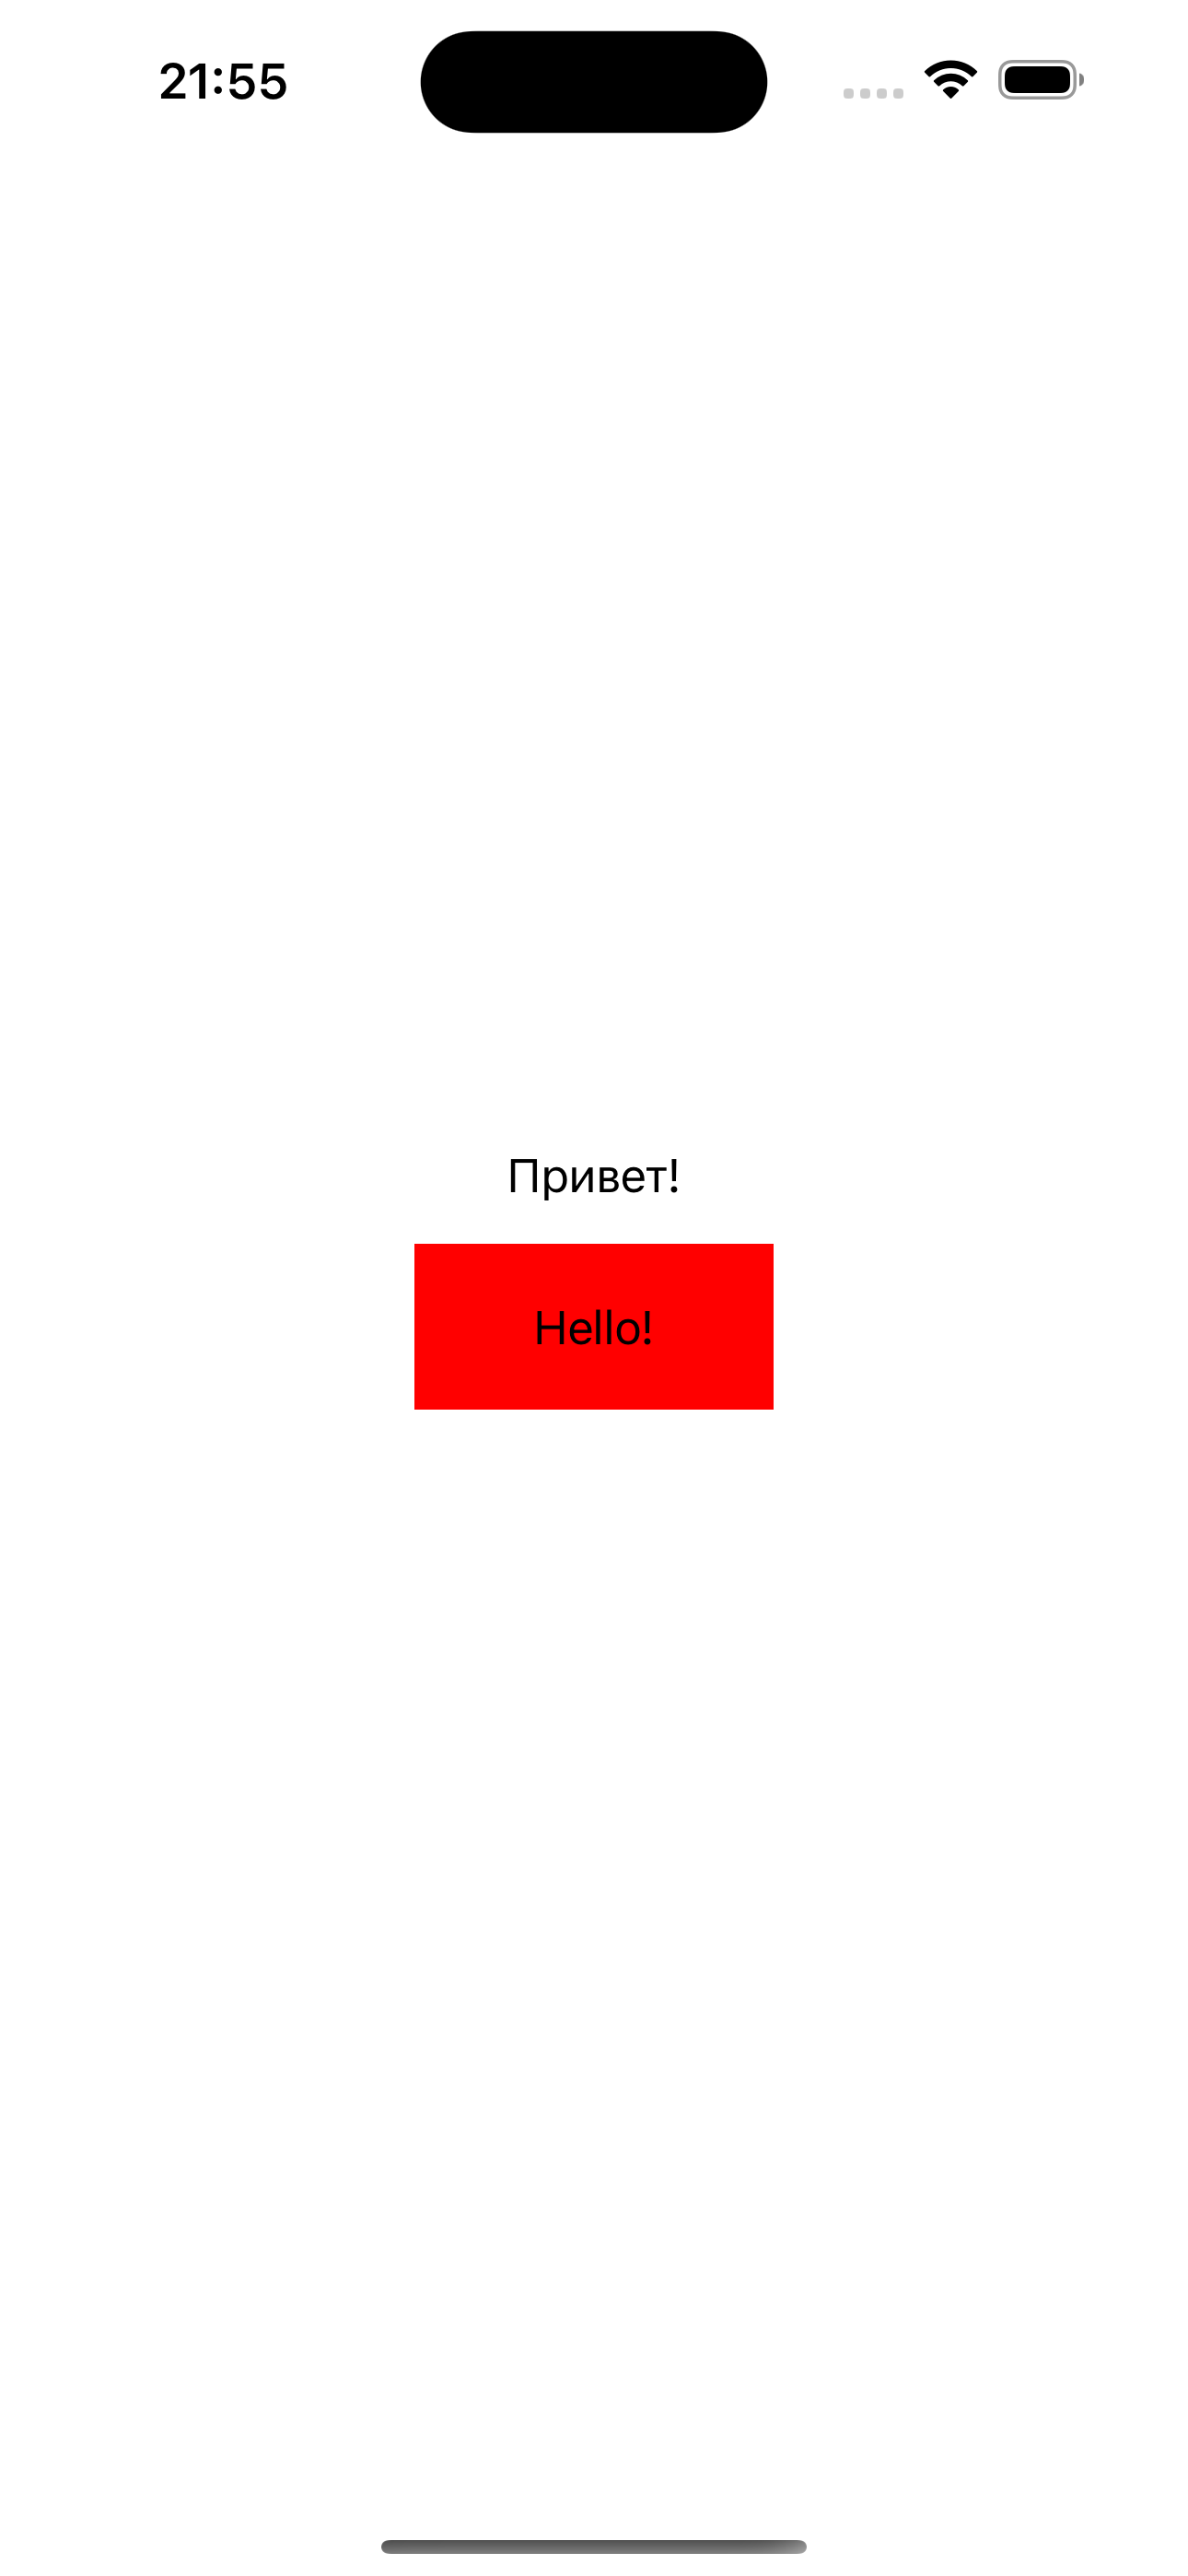
\includegraphics[scale=0.1]{img/example-after.png}
	\caption{Интерфейс после внесения изменений}
	\label{fig:example-after}
\end{figure}

\subsubsection{Тестирование}
Разработанное программное обеспечение должно гарантировать корректное отображение задаваемых UI--элементов.
Для этого было проведено snapshot--тестирование, в рамках которого эталонные скриншоты экрана сравниваются с актуальным скриншотами, которые получаются во время прогона тестов.
В качестве эталонных скриншотов используются представления, сверстанные с помощью фреймворка UIKit.
Для выполнения тестирования была использована библиотека SnapshotTesting, предоставляющая весь необходимый для создания snapshot--тестов функционал.

В таблицах 2 --- 5 представлен набор тестов, а также результат их выполнения.
Каждый тест предполагает наличие фонового UIView белого цвета.

\begin{table}[!htb]
 \label{table:tests1}
 \begin{center}
  \caption{Результаты snapshot--тестирования}
 \begin{tabular}{|p{0.6cm}|p{10cm}|p{5cm}|}
  \hline
   \bfseries № & \bfseries Описание теста & \bfseries Результат \\ \hline
   1 & UIView черного цвета, занимает верхнюю половину экрана & Тест пройден успешно  \\ \hline
   2 & UIView красного цвета, занимает нижнюю половину экрана & Тест пройден успешно  \\ \hline
   3 & UIView синего цвета, занимает левую половину экрана  & Тест пройден успешно  \\ \hline      
   4 & UIView оранжевого цвета, занимает правую половину экрана  & Тест пройден успешно  \\ \hline
   5 & UIView фиолетового цвета, ширина 20, высота 20, левая граница --- левая граница экрана, верхняя граница --- верхняя граница экрана & Тест пройден успешно  \\ \hline
   6 & UIView зеленого цвета, ширина 20, высота 20, правая граница --- правая граница экрана, верхняя граница --- верхняя граница экрана & Тест пройден успешно  \\ \hline
   7 & UIView серого цвета, занимает верхнюю половину экрана + UIView розового цвета, занимает нижнюю половину экрана & Тест пройден успешно  \\ \hline
   8 & UIView серого цвета, занимает левую половину экрана + UIView розового цвета, занимает правую половину экрана & Тест пройден успешно  \\ \hline
   9 & UILabel, цвет фона --- красный, текст --- <<Привет>>, отступ 100 от верхней границы экрана, отступ 100 от правой границы экрана, ширина и высота 100 & Тест пройден успешно  \\ \hline
  \end{tabular}
 \end{center}
\end{table}

\begin{table}[!htb]
 \label{table:tests2}
 \begin{center}
  \caption{Результаты snapshot--тестирования --- продолжение}
 \begin{tabular}{|p{0.6cm}|p{10cm}|p{5cm}|}
  \hline
   \bfseries № & \bfseries Описание теста & \bfseries Результат \\ \hline
   10 & UILabel, цвет фона --- красный, текст --- <<Привет>>, выравнивание текста по правому краю, отступ 100 от верхней границы экрана, отступ 100 от правой границы экрана, ширина и высота 100 & Тест пройден успешно  \\ \hline
   11 & UILabel, цвет фона --- красный, текст --- <<Привет>>, выравнивание текста по левому краю, отступ 100 от верхней границы экрана, отступ 100 от правой границы экрана, ширина и высота 100 & Тест пройден успешно  \\ \hline
   13 & UIView оранжевого цвета, занимает правую половину экрана + дочерний UILabel, цвет фона --- красный, текст --- <<Привет>>, выравнивание текста по правому краю, отступ 100 от верхней границы UIView, отступ 100 от правой границы UIView, ширина и высота 100 & Тест пройден успешно  \\ \hline
   14 & UIView оранжевого цвета, занимает правую половину экрана + дочерний UILabel, цвет фона --- красный, текст --- <<Привет>>, выравнивание текста по правому краю, отступ -100 от нижней границы UIView, отступ 100 от левой границы UIView, ширина и высота 100 & Тест пройден успешно  \\ \hline
  \end{tabular}
 \end{center}
\end{table}

\begin{table}[!htb]
 \label{table:tests3}
 \begin{center}
  \caption{Результаты snapshot--тестирования --- продолжение}
 \begin{tabular}{|p{0.6cm}|p{10cm}|p{5cm}|}
  \hline
   \bfseries № & \bfseries Описание теста & \bfseries Результат \\ \hline
   15 & UIView оранжевого цвета, занимает правую половину экрана + дочерний UILabel, цвет фона --- красный, текст --- <<Привет>>, выравнивание текста по правому краю, отступ 100 от нижней границы UIView, отступ 100 от левой границы UIView, ширина и высота 100 & Тест пройден успешно  \\ \hline
   16 & UIView красного цвета, 75\% экрана + дочерний UIView зеленого цвета, 50\% экрана + дочерний UIView коричневого цвета, 25\% экрана  & Тест пройден успешно  \\ \hline   
   17 & UIView красного цвета, 75\% экрана + дочерний UIView зеленого цвета, 50\% экрана + дочерний UIView коричневого цвета, 25\% + дочерний UIView синего цвета, 12\% экрана  & Тест пройден успешно  \\ \hline
   18 & UIView красного цвета, 75\% экрана + дочерний UIView зеленого цвета, 50\% экрана + дочерний UIView коричневого цвета, 25\% + дочерний UIView синего цвета, 12\% экрана + дочерний UIView оранжевого цвета, 6\% экрана  & Тест пройден успешно  \\ \hline
   19 & UIView красного цвета, 75\% экрана + дочерний UIView зеленого цвета, отступ 100 от правой границы родителя, ширина и высота 100 и второй дочерний UIView коричневого цвета, отступ -100 от левой границы родителя, ширина и высота 100 & Тест пройден успешно  \\ \hline
     \end{tabular}
 \end{center}
\end{table}

\begin{table}[!htb]
 \label{table:tests4}
 \begin{center}
  \caption{Результаты snapshot--тестирования --- продолжение}
 \begin{tabular}{|p{0.6cm}|p{10cm}|p{5cm}|}
  \hline
   \bfseries № & \bfseries Описание теста & \bfseries Результат \\ \hline
   20 & UIView красного цвета, 75\% экрана + дочерний UIView зеленого цвета, отступ 100 от правой границы родителя, ширина и высота 50, второй дочерний UIView коричневого цвета, отступ -100 от левой границы родителя, ширина и высота 50, третий дочерний UIView зеленого цвета, отступ 10 от верхний границы родителя, ширина и высота 50 & Тест пройден успешно  \\ \hline
   21 & UIView красного цвета, 75\% экрана + дочерний UIView зеленого цвета, отступ 100 от правой границы родителя, ширина и высота 50, второй дочерний UIView коричневого цвета, отступ -100 от левой границы родителя, ширина и высота 50, третий дочерний UIView зеленого цвета, отступ 10 от верхний границы родителя, ширина и высота 50 + дочерний UILabel, цвет фона --- красный, текст --- <<Привет>>, выравнивание текста по правому краю, отступ 10 от верхней границы родителя & Тест пройден успешно  \\ \hline  \end{tabular}
 \end{center}
\end{table}

\subsection*{Вывод}

В данном разделе был обоснован выбор средств программной реализации предлагаемого метода, описан формат входных и выходных данных. 
Разработано программное обеспечение, реализующее представленный метод, приведен пример работы программы, выполнено тестирование, а также описан способ обращения к программе.

\pagebreak